\subsection{Der core-Ordner}
Die Abbildung \ref{fig:core-sturktur} bietet eine Übersicht des Ordnerinhaltes und der inneren Abhängigkeiten.
Dem Anhang ist das Diagram D2\_Core.html beigefügt, welches eine detailliertere Darstellung der Abhängigkeit enthält.
Die Tabelle \ref{table:coreMap} kategorisiert den Quelletext des Ordners in Bausteine.

\begin{figure}[H]
    \centering
    \caption{Übersicht der Strukturierung des Ordners \lstinline|core|}
    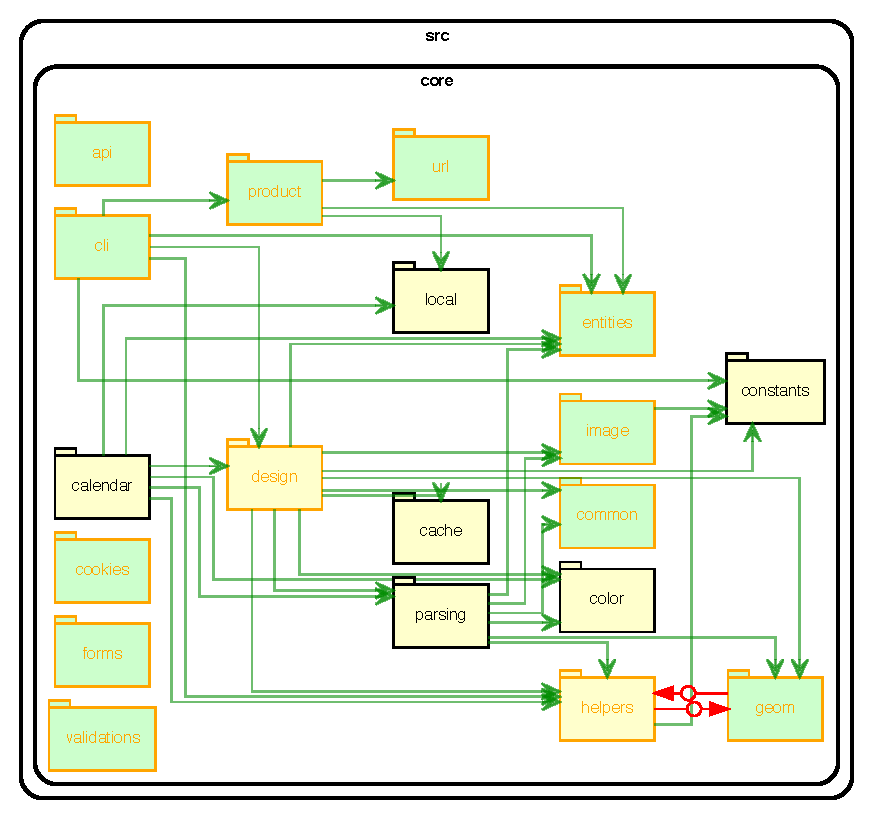
\includegraphics[width=.7\textwidth]{diagrams/Ist-Architektur/core-graph.pdf}
    \label{fig:core-sturktur}
\end{figure}

\begin{filecontents}[overwrite]{\jobname-core-map.tex}
\begin{longtable}{r@{\hspace{3mm}}lX}
    \caption{Die Kategorisierung des Quelletexts innerhalb \lstinline|core| in Bausteine} \\
    \label{table:coreMap}
    \rownumbereset
    & \textbf{Baustein} & \textbf{Quelltext} \\
    \hline

    \hline
    \rownumber & API-Kommunikation & api/* \\
    \hline 

    \rownumber & Anwenderregistrierung 
    & forms/* \\
    \hline 

    \rownumber & Bildverarbeitung 
    & image/* \\
    \hline 

    \rownumber & Cache 
    & cache/Cache.ts \\
    \hline 

    \rownumber & Cookie-Verarbeitung 
    & cookies/handler.ts \\
    \hline 

    \rownumber & Design-Migration 
    & design/DesignCompatibility.ts \\
    \hline 

    \rownumber & Design-Parser 
    & design/designParser/* \\
    \hline 

    \rownumber & Design-Serialisierung 
    & design/DesignSerializer.ts \\
    \hline 

    \rownumber & Designbearbeitung 
    & design/ITextSelection.ts \\
    & & design/index.ts \\
    & & helpers/RotationRaster.ts \\
    \hline

    \rownumber & Designobjekt-Transformation
    & design/transformation/* \\
    & & design/DesignItemFunctions.ts \\
    \hline 

    \rownumber & Designobjekterzeugung 
    & design/DesignItemBuilder.ts \\
    \hline 

    \rownumber & Designstruktur 
    & design/DesignIterator.ts \\
    & & entities/FDDesign.ts \\
    \hline 

    \rownumber & Farbstruktur 
    & color/* \\
    & & validations/ColorValidations.ts \\
    \hline 

    \rownumber & Formularverarbeitung 
    & forms/FormParser.ts \\
    \hline 

    \rownumber & Fotogalerie 
    & common/Gallery.ts \\
    \hline 

    \rownumber & Grafische-Oberfläche 
    & validations/\\ 
    & & common/MenuOption.ts \\
    & & common/\\ 
    \hline 

    \rownumber & JavaScript-Erweiterung 
    & common/index.ts \\
    & & common/UserAgent.ts \\
    & & helpers/Clone.ts \\
    & & helpers/FDArrayHelper.ts \\
    & & helpers/index.ts \\

    \hline 
    \rownumber & Kalendariumserzeuger 
    & calendar/* \\
    & & common/Calendar.ts \\
    \hline 

    \rownumber & Kalenderkonfigurator 
    & entities/DateInterfaces.ts \\
    \hline 

    \rownumber & Kurzinformation 
    & helpers/CalculateTooltipPos.ts \\


    \rownumber & Mathematik 
    & geom/* \\
    & & helpers/FDMath.ts \\
    & & helpers/deCasteljau.ts \\
    \hline 

    \rownumber & Maßeinheit-Konverter 
    & helpers/MeasureUtils.ts \\
    \hline 

    \rownumber & Produktstruktur 
    & product/* \\
    & & entities/product/* \\
    \hline 

    \rownumber & SVG-Konverter 
    & design/DesignSvgCreator.ts \\
    \hline 

    \rownumber & SVG-Parser 
    & parsing/svgParsing.ts \\
    \hline 

    \rownumber & Schriftverarbeitung 
    & design/FontFunctions.ts \\
    & & entities/IFontData.ts \\
    \hline 

    \rownumber & Speicherkomponente 
    & validations/\\ 
    \hline 

    \rownumber & Textschlüsselsammlung 
    & local/index.ts \\
    \hline 

    \rownumber & URL-Verarbeitung 
    & url/* \\
    \hline 

    \rownumber & Vorlagekonverter 
    & design/designTemplate/* \\
    & & cli/* \\
    \hline 

    \rownumber & XML-Parser 
    & parsing/xmlParsing.ts \\
    \hline 

\end{longtable}
\end{filecontents}
\LTXtable{\linewidth}{\jobname-core-map.tex}